% 2009 年湖北卷理科第 18 题：四棱锥 S-ABCD。
% 来源 PDF：2009湖北理.pdf，SHA-256 a78cef31900f38a49e4940931067c750cdff63c9d4dab40c72dbd09e56e80f3a。
% 原页：第 2 页第 1 栏上部，书页码 524。
% 重绘依据：底面 ABCD 为正方形，SD⊥底面，故 SD 画成竖直线并落到底面顶点 D 上；
%   D 在锥体内部，SD、DA、DC、AC 均被遮挡，画虚线；SA、SB、SC、AB、BC 为可见
%   棱，画实线。原页未在图上标出点 E（E 在 SD 上，由题面给出 DE=λa），故此处亦
%   不添标 E，保持与原页一致。
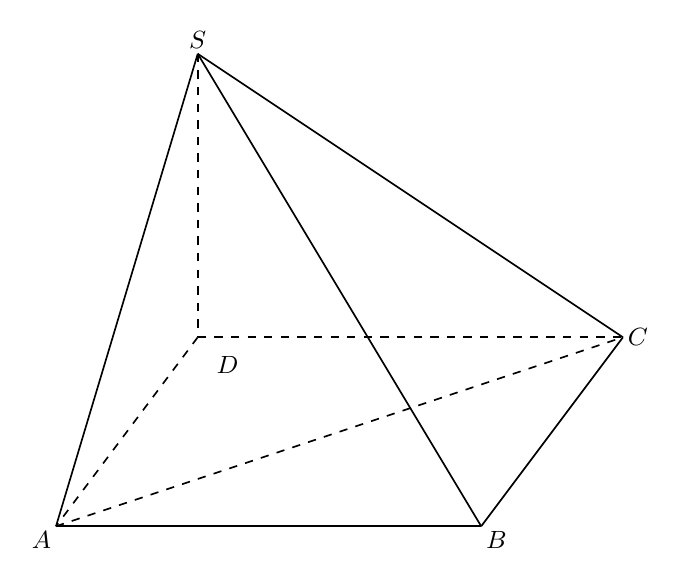
\begin{tikzpicture}[semithick, every node/.style={inner sep=1.5pt, font=\small}]
  \coordinate (A) at (0.2,1.2);
  \coordinate (B) at (5.6,1.2);
  \coordinate (C) at (7.4,3.6);
  \coordinate (D) at (2.0,3.6);
  \coordinate (S) at (2.0,7.2);

  % 可见棱
  \draw (S) -- (A);
  \draw (S) -- (B);
  \draw (S) -- (C);
  \draw (A) -- (B);
  \draw (B) -- (C);

  % 被遮挡的棱
  \draw[dashed] (S) -- (D);
  \draw[dashed] (D) -- (A);
  \draw[dashed] (D) -- (C);
  \draw[dashed] (A) -- (C);

  % 标签
  \node[above] at (S) {$S$};
  \node[below right=5pt] at (D) {$D$};
  \node[below left] at (A) {$A$};
  \node[below right] at (B) {$B$};
  \node[right] at (C) {$C$};
\end{tikzpicture}
